\begin{figure}[h]
    \centering
    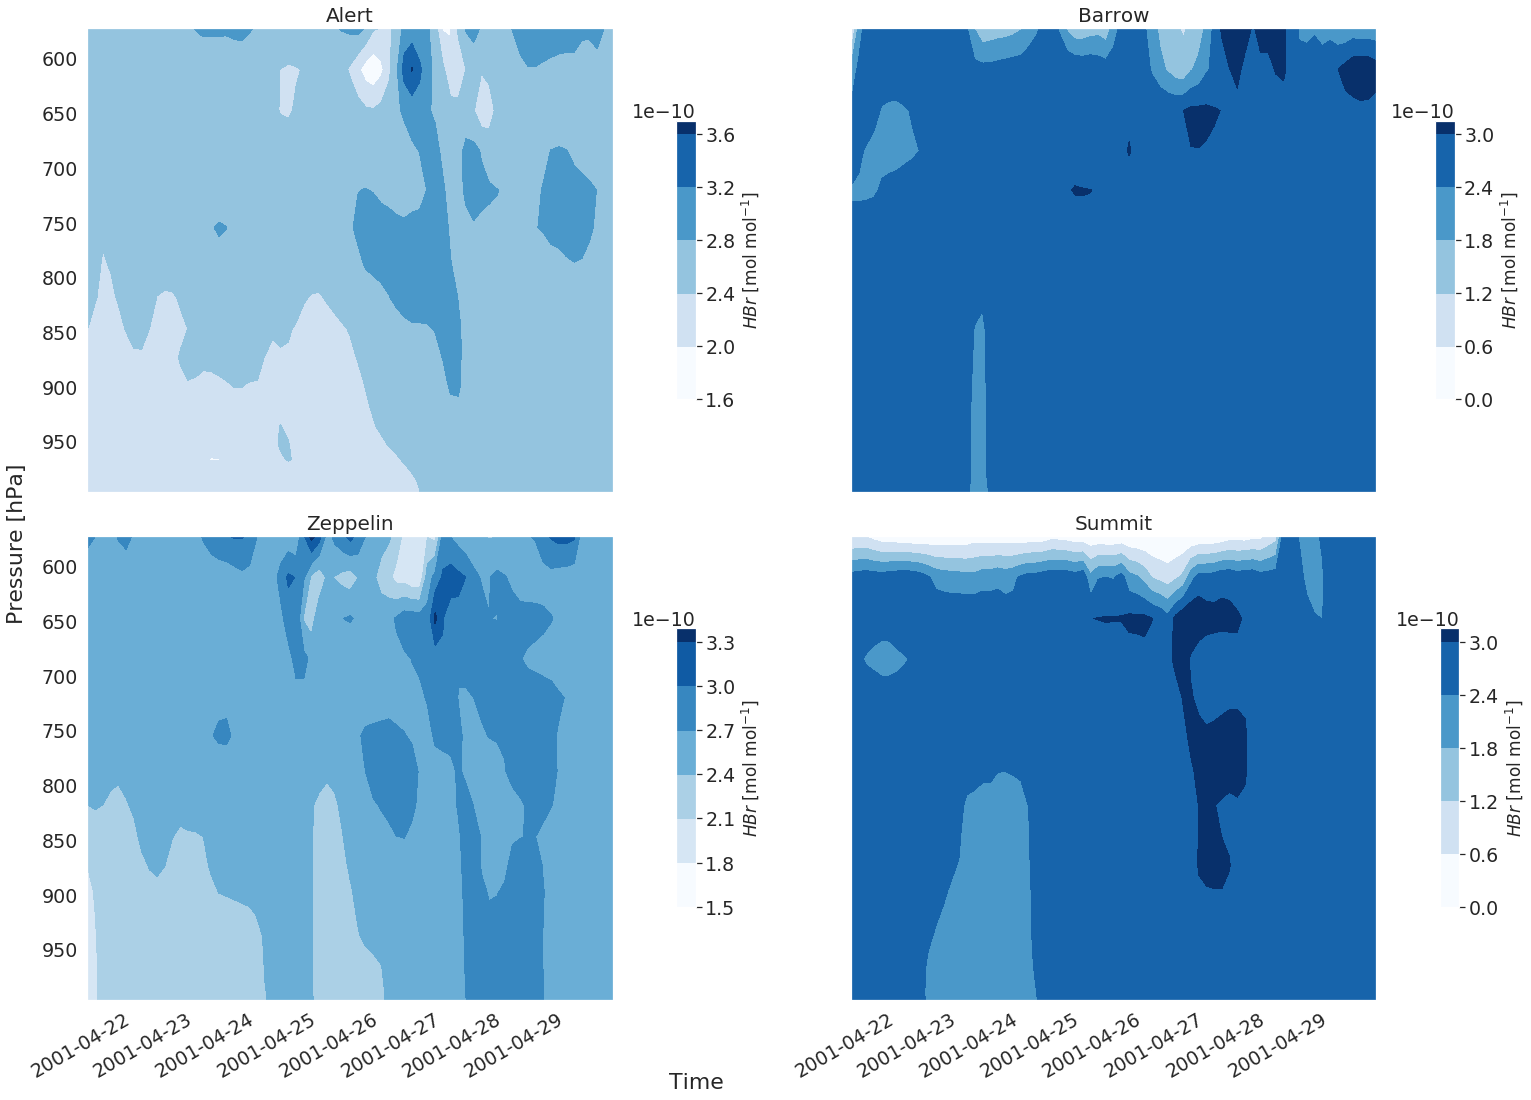
\includegraphics[width=\linewidth]{Chapter6_Results/images/vertHBr_HTWO_step3.png}
    \caption{Mixing ratio ($mol mol^{-1}$) of \chem{HBr} in the model layers up to $\sim 600 hPa$ at the four different stations Alert (top left), Barrow (top right), Zeppelin (lower left) and Summit (lower right) in April, 2001. The result is from the test including hard-coded photodissociation rates as well as a new (high) Henry-coefficient at HTWO resolution}
    \label{fig:vertHBr_HTWO_step3}
\end{figure}